\subsection{Who is our target user?}
\textit{Magpie's} primary target is Urban Planners. Urban Planners are
professionals responsible for the development of cities and towns, focusing on
the efficient use of land, infrastructure planning, and the creation of
sustainable and resilient communities. (\cite{fischler2012fifty}) Our secondary
target is any non-expert user who is interested in amenities planning, and this
includes but is not limited to the following: Sustainability Advocates,
Commuters, Event Planners, Journalists, Political Advisors, and Parking
Companies.

These personas were developed on basis of a combination of real-life people who
are known to our team, as well as based on research into the goals and needs of
people in these professions

\subsubsection{Primary Persona - Michael O'Brien}
O'Brien is a 48-year-old Urban Planning Specialist at Dublin City Council,
deeply committed to enhancing his hometown of Lusk. He specializes in
sustainable urban development, integrating smart technologies with traditional
planning principles, and has contributed to notable projects like Dublin's cycle
lane network. He represents our primary target user.

Michael is currently working on the expansion of Dublin's cycle lane network
southbound. He is facing some challenges because the maps provided by Dublin
city council are static and don't show crucial information such as public
facilities and amenities. The datasets he's been accessing seem out of date and
not comprehensive at all. Michael needs a tool that allows him to interact with
a map that contains key data on public facilities and amenities, as well as
options to extract that information for analysis and planning.

%michael user persona
\begin{figure}[htbp]
    \centering{}{}
    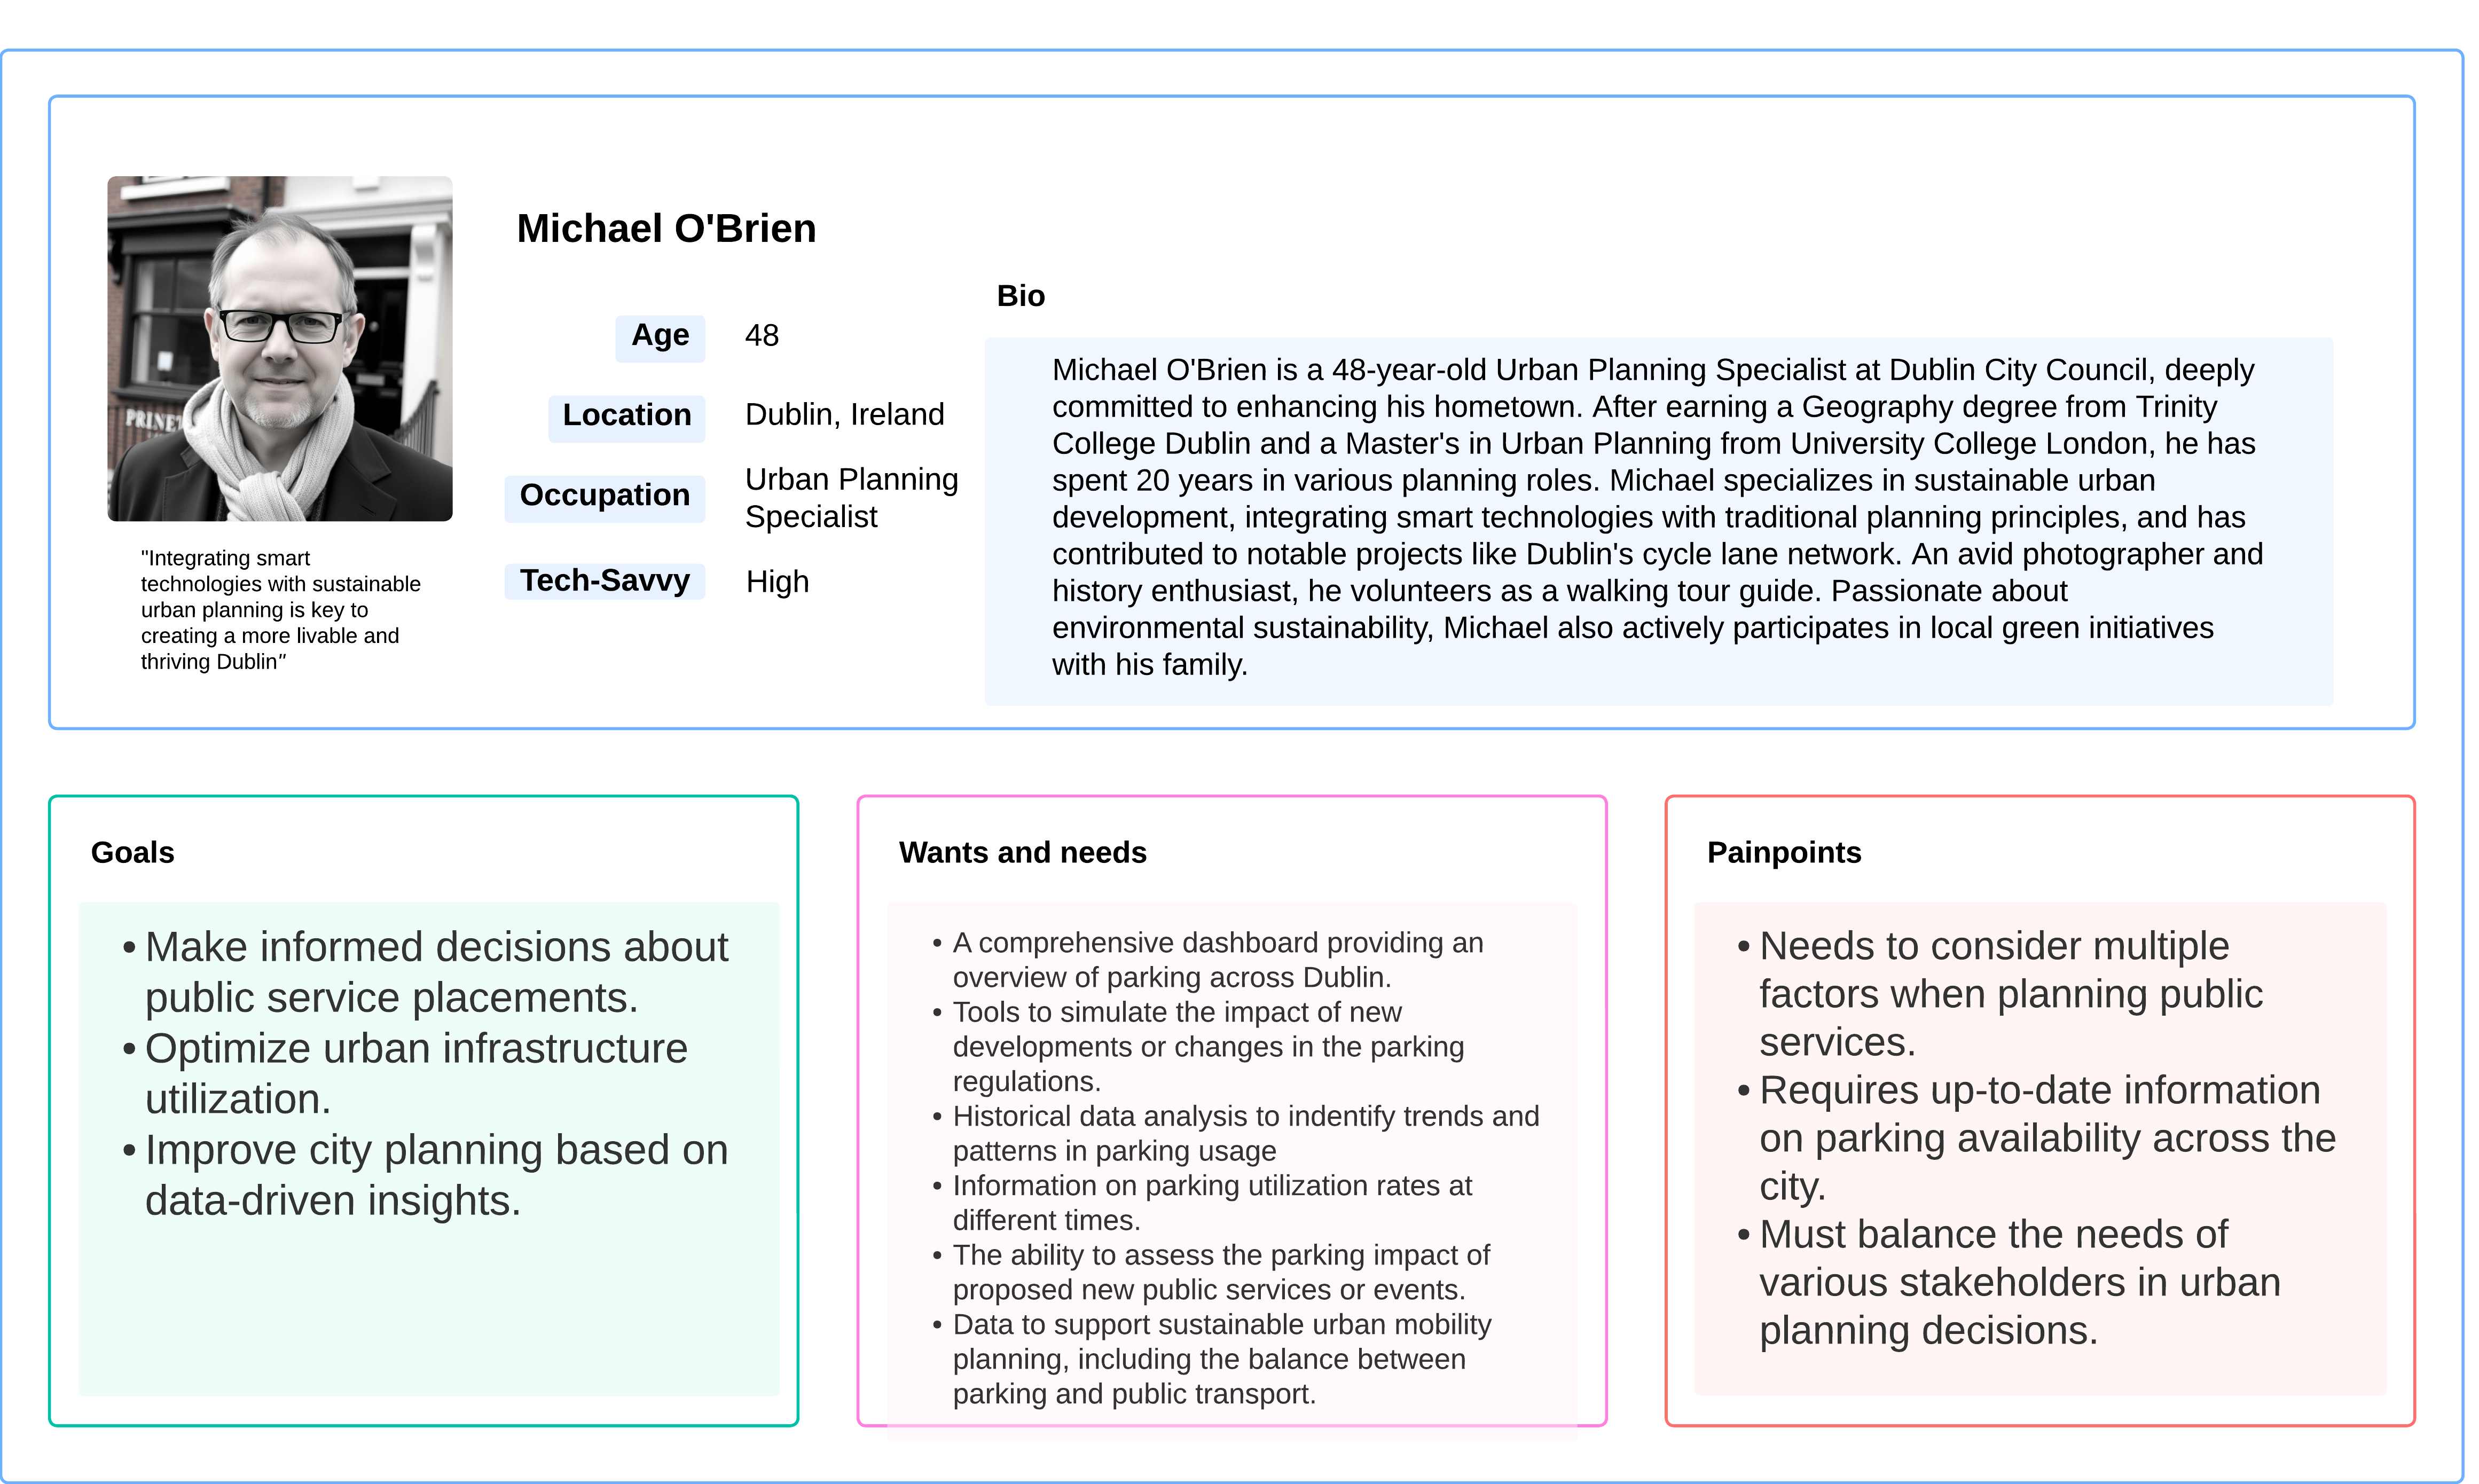
\includegraphics[width=0.8\textwidth]{images/michael-obrien-userpersona.png}
    \caption{User persona - Michael O'Brien}
\end{figure}

\subsubsection{Secondary Persona - Sarah Thompson}
Sarah thompson is a 35 year old CEO of an event's planning company based in
Dublin, Ireland. She specializes in corporate events and weddings, and is known
for creating memorable experiences while addressing key logistical challenges
such as venue selection, catering, accessibility and transportation. She
represents our secondary target user.

%sarah user persona
\begin{figure}[htbp!]
    \centering{}{}
    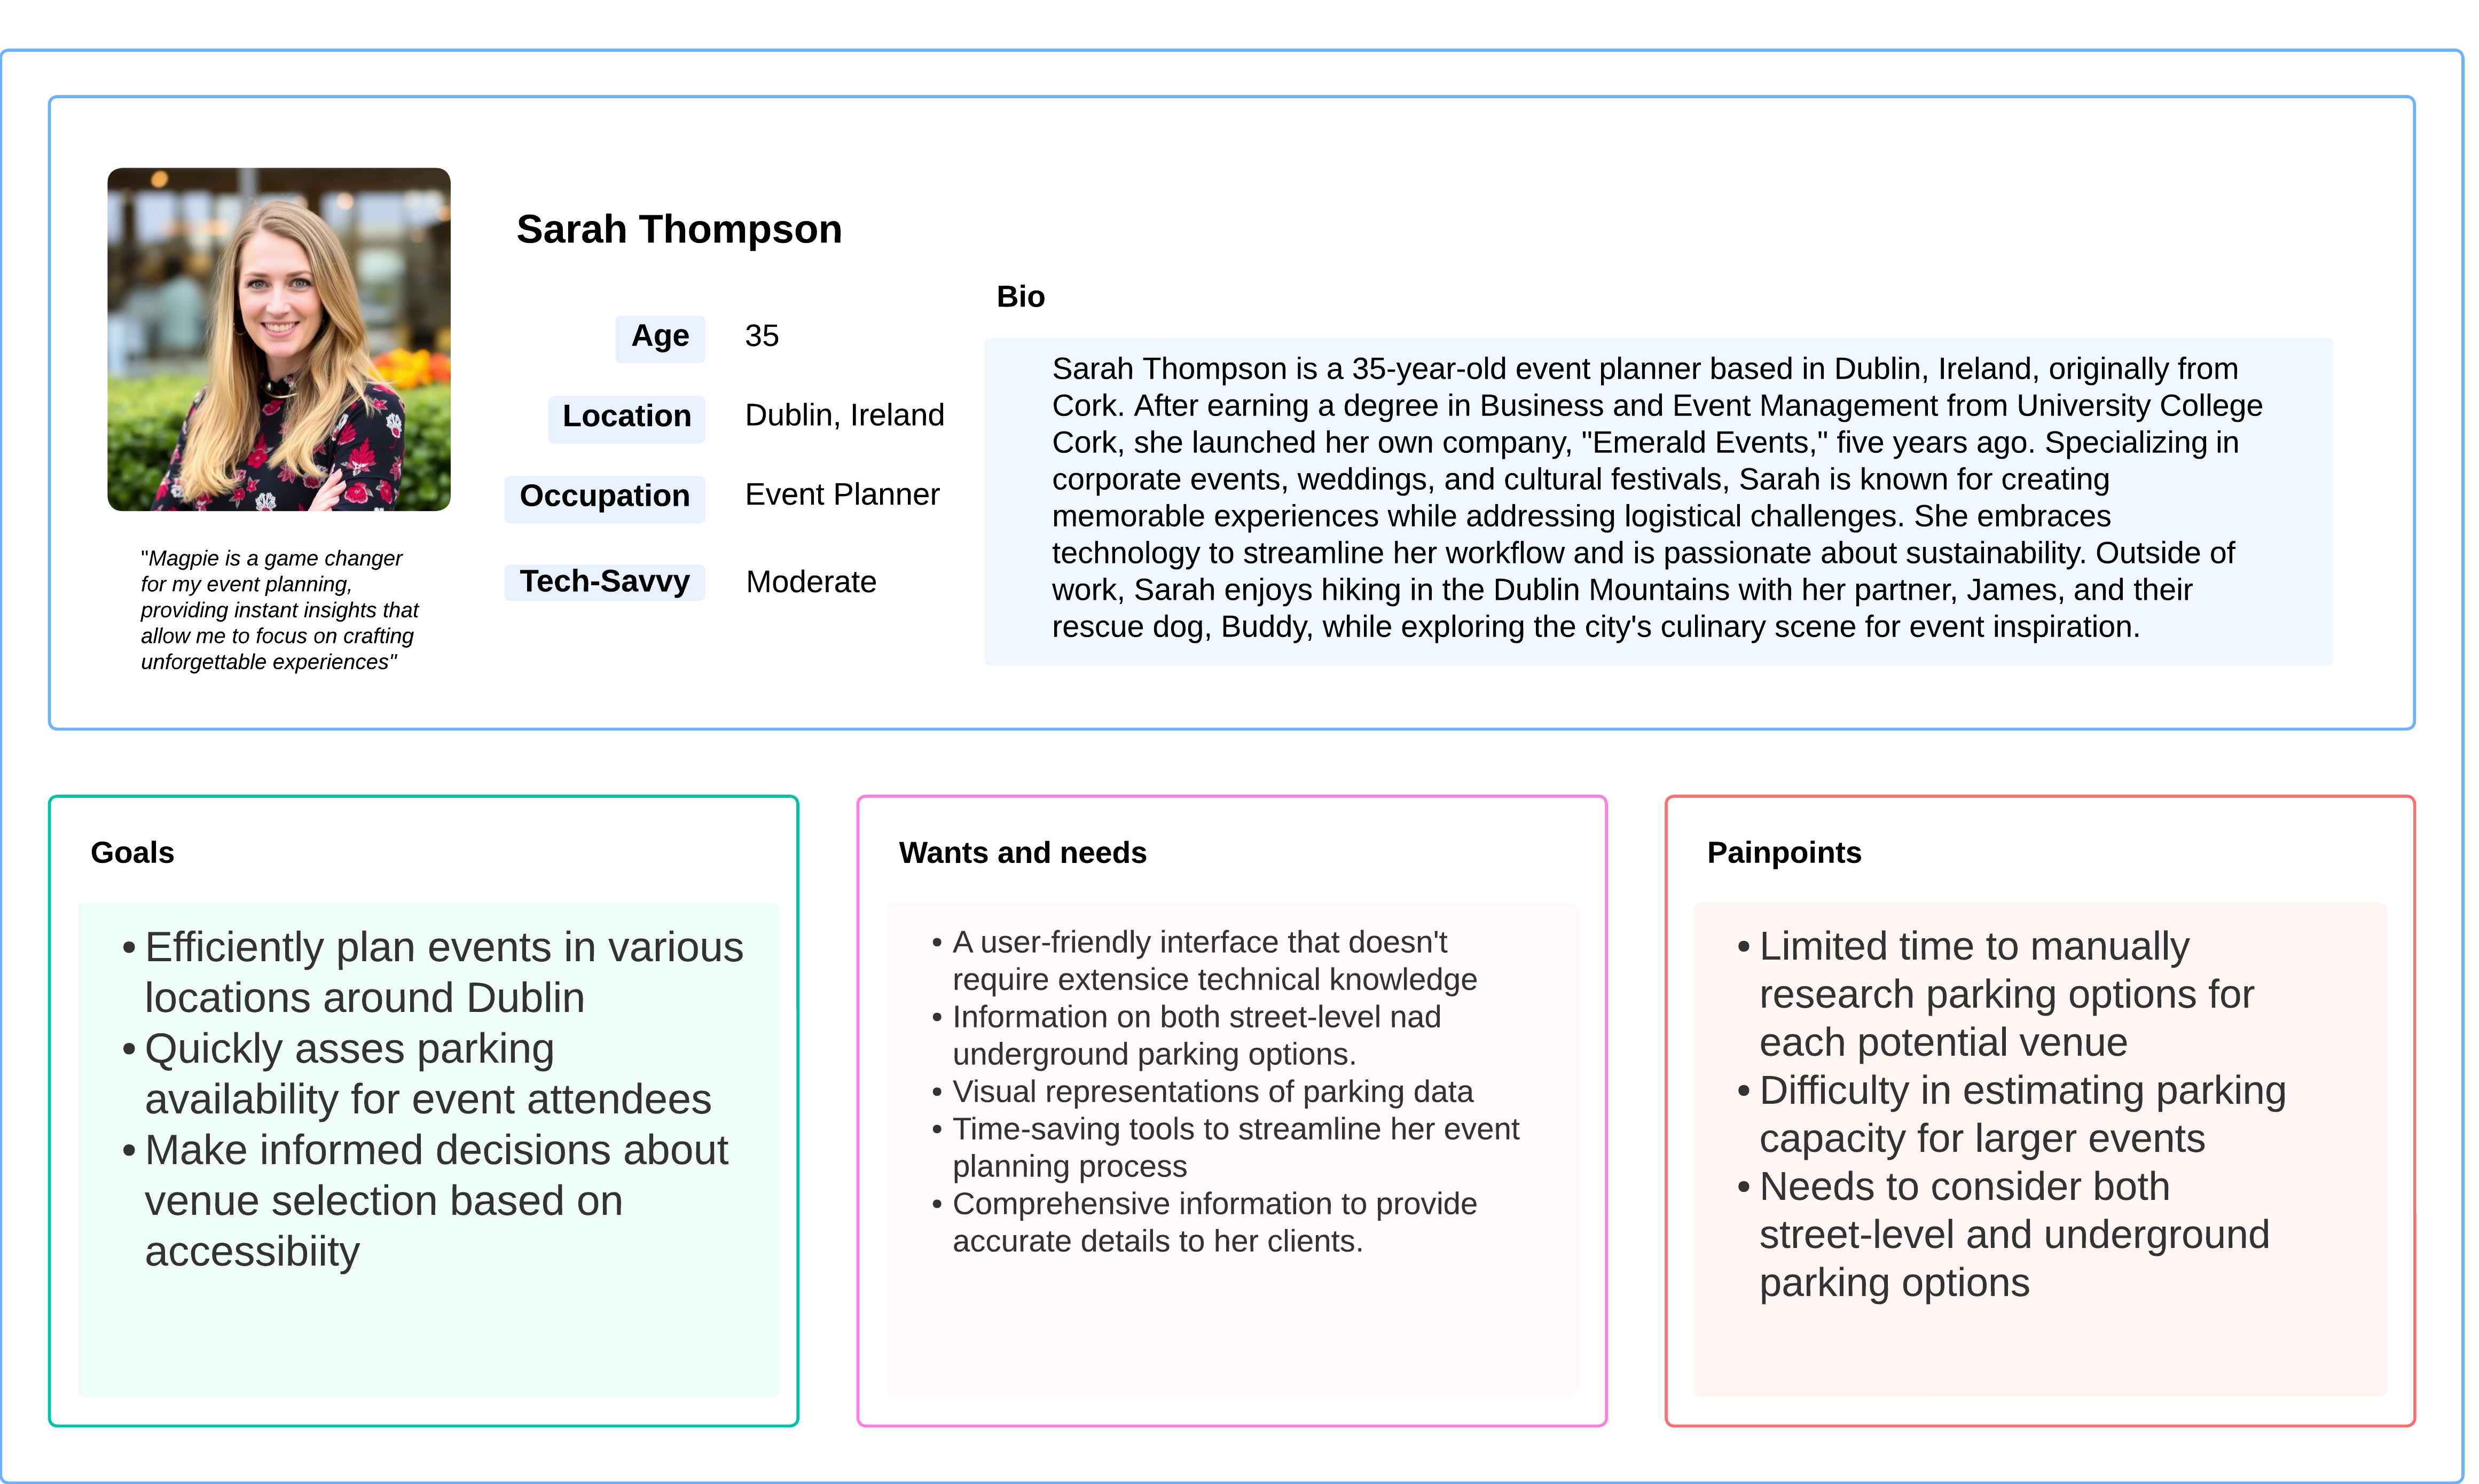
\includegraphics[width=0.8\textwidth]{images/sarah-thompson-userpersona.png}
    \caption{User persona - Sarah Thompson}
\end{figure}

\newpage{}

Currently, she faces many challenges planning events within Dublin city. She has
limited time to manually research transport and parking options and to visually
assess the accessibility of a possible venue. She's looking for a tool that will
give her a visual overview of transportation and parking options in an area,
with additional information on their location  \& their quantity. She also needs
something quick and easy to use.

\subsection{Why are they important?}
Urban Planners are crucial for the holistic development of cities and towns.
(\cite{jha2021review})They ensure that urban development is sustainable,
balancing economic growth and environmental protection. (\cite{lei2021urban})
Urban planners guide cities towards more efficient uses of land, better
transport systems, and overall increasing the quality of life of residents.
(\cite{janpavle2022importance})

By planning for current and future needs, Urban Planners help mitigate urban
challenges such as congestion, pollution, and lack of infrastructure. Their role
is essential for ensuring that urban areas can meet the demands of growing
populations, while maintaining standard of living and environmental
sustainability.

\subsection{What problem are we solving?}
Urban Planners often face challenges with accessing and analysing data. Data is
typically siloed, making it difficult to access and analyse.
(\cite{duivenvoorden2021managing})

We aim to provide Urban Planners with a tool that allows them to access this
information in a single, easy to use, platform. This will allow Urban Planners
to streamline the initial phases of their work, decreasing the time spent on
data collection and increasing the time spent on analysis and decision making.

\subsection{Market analysis}
The identification of our target user was made possible through exploratory work
done at the beginning of the project timeline. A research survey was conducted
using Microsoft Forms, sent out to county councils, planners, firms and the
TUDublin mailing list, to answer key demographic \& product questions:
\begin{enumerate}
    \item{Who is our primary target user?}
    \item{What kind of amenity data do they access and how?}
    \item{What devices/tools do they primarily use?}
    \item{Are they satisfied with those tools?}
    \item{Would they consider Magpie useful in filling the gaps in their toolset?}
\end{enumerate}

\newpage{}

\subsubsection{Demographic data}
This first section of the survey covered demographic data, to allow us to build a profile for the respondents. Personal identifiable information was not collected for the purposes of anonymity.

We had a total of 118 respondents, which we divided into 2 categories:

\emph{User A}: Respondents who did not use amenity data in their work = \textbf{88 users}.
\emph{User B}: Respondents who used amenity data in their work = \textbf{30 users}.
Splitting the respondents allows us to better analyse the answers in the context of if they belong to our primary or our secondary target user group.

Both user groups were evenly distributed in employment sector and counties they work in, as illustrated in the figures below.

%user sector distribution
\begin{figure}[htbp]
    \centering{}{}
    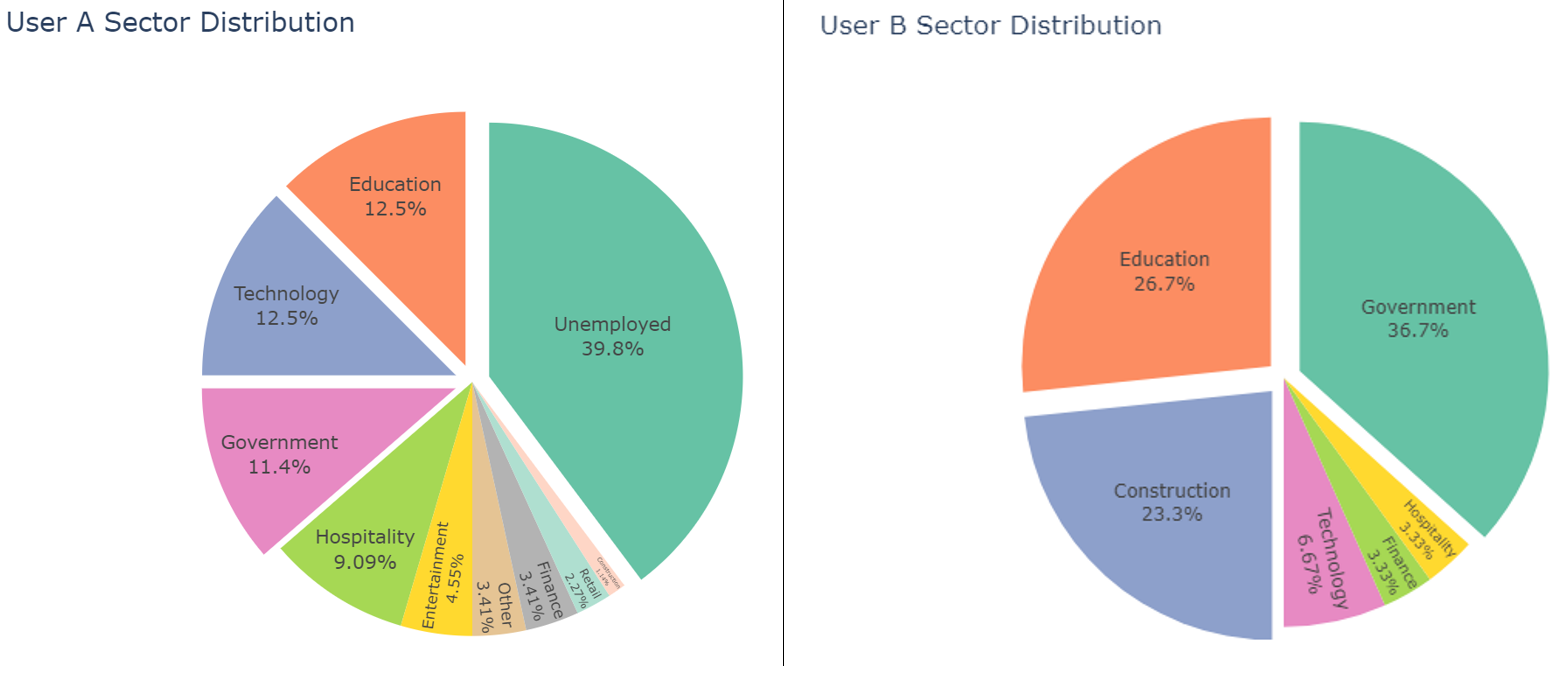
\includegraphics[width=0.8\textwidth]{images/mr-sector-distribution.png}
    \caption{Market analysis - User Sector Distribution}
\end{figure}

%user sector distribution
\begin{figure}[htbp]
    \centering{}{}
    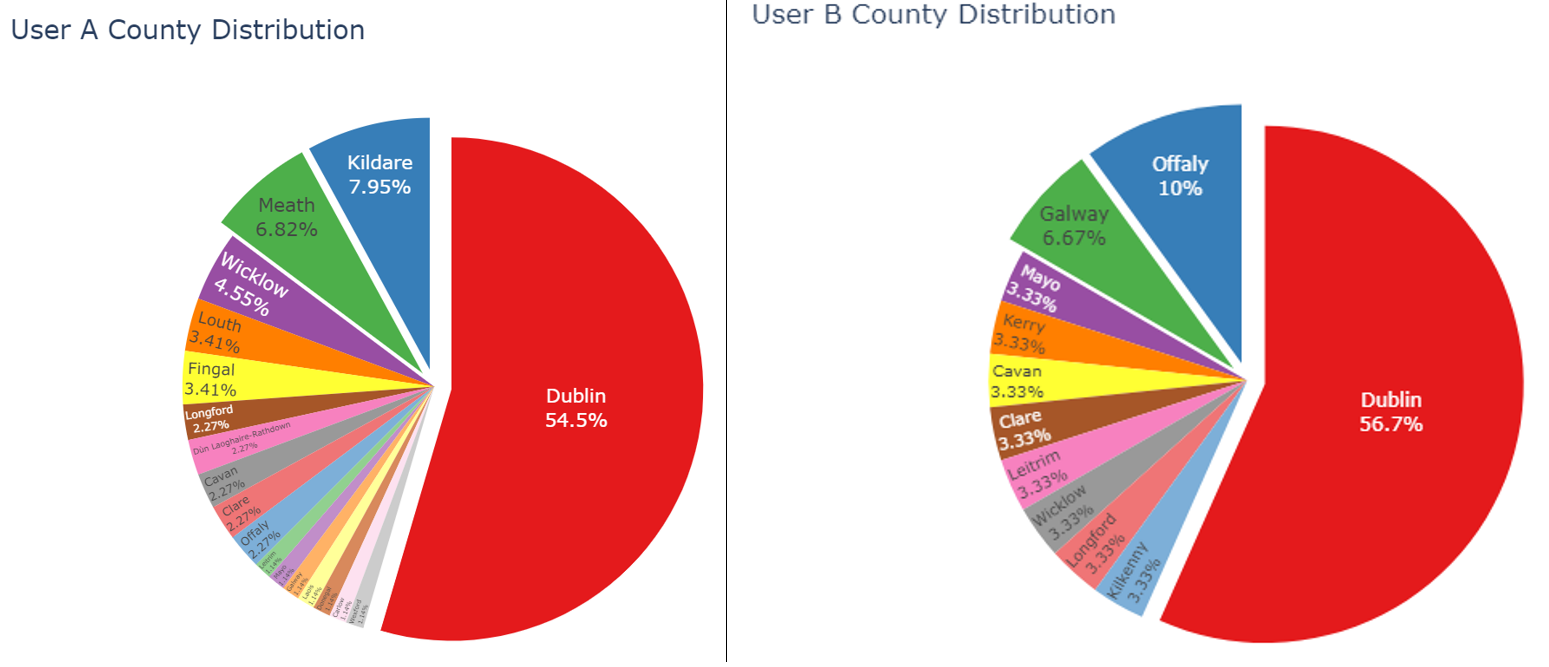
\includegraphics[width=0.8\textwidth]{images/mr-county-distribution.png}
    \caption{Market analysis - User County Distribution}
\end{figure}

\newpage{}

\subsubsection{Amenity data}
This section specifically questions respondents in the User B group on their use of amenity data in their work.

We can see that the most common amenity data accessed is transportation.

%amenity data type accessed
\begin{figure}[htbp]
    \centering{}{}
    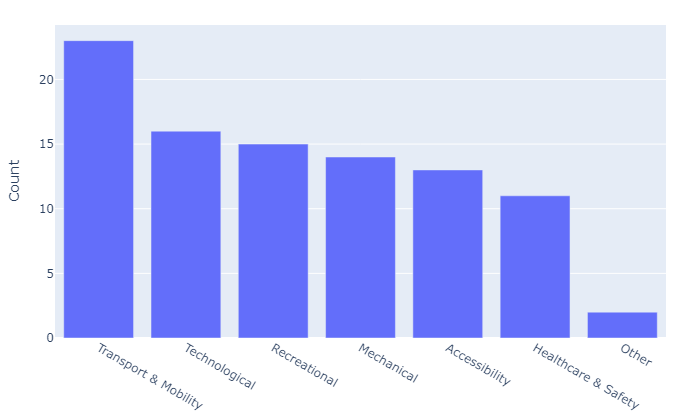
\includegraphics[width=0.8\textwidth]{images/mr-userb-amenity.png}
    \caption{Market analysis - User B Amenity Data Type Distribution}
\end{figure}

\subsubsection{Devices \& Tools}
This section looks at the devices used by both users groups, as well as the
applications or tools they are using to access amenity data.

User A was specifically questioned on which device they use for navigation and
at what frequency.

%device + freq user A
\begin{figure}[htbp]
    \centering{}{}
    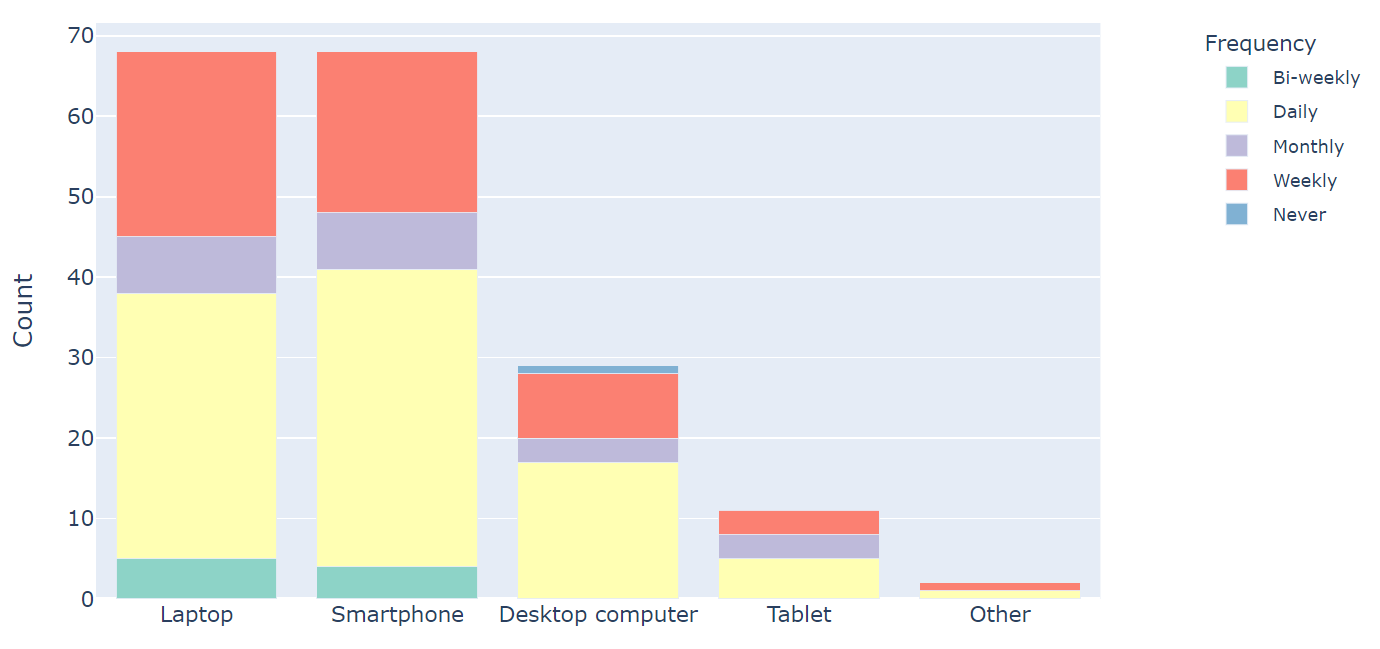
\includegraphics[width=0.8\textwidth]{images/mr-usera-device-freq.png}
    \caption{Market analysis - User A Preferred device \& Usage frequency}
\end{figure}

User B was specifically questioned on which device they use for their day-to-day
work, as well as what tool they are currently using to access amenity data.

%device + freq user B
\begin{figure}[htbp]
    \centering{}
    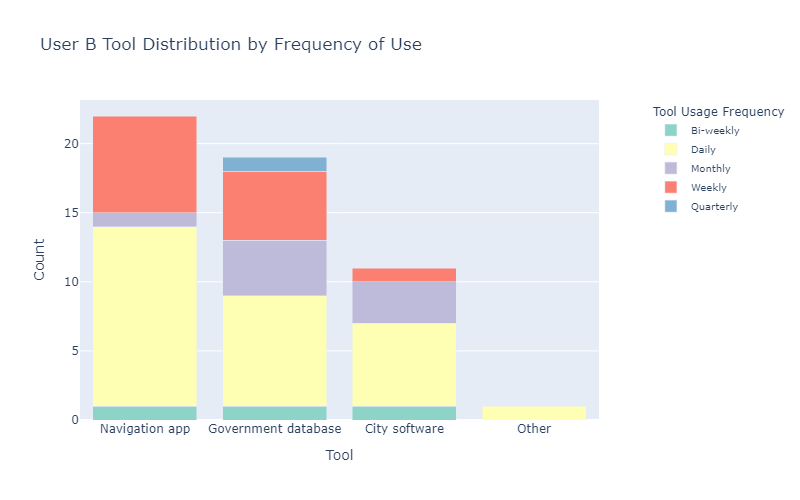
\includegraphics[width=0.8\textwidth]{images/mr-userb-tool-freq.png}
    \caption{Market analysis - User B Tool type \& Usage frequency}
\end{figure}

User B were also questioned on their satisfaction with their current tool. More
than 50\% of respondents said they weren't completely satisfied, citing
incomplete information, lack of user friendliness and poor speed as reasons.

%tool + satisfaction user B
\begin{figure}[htbp]
    \centering{}
    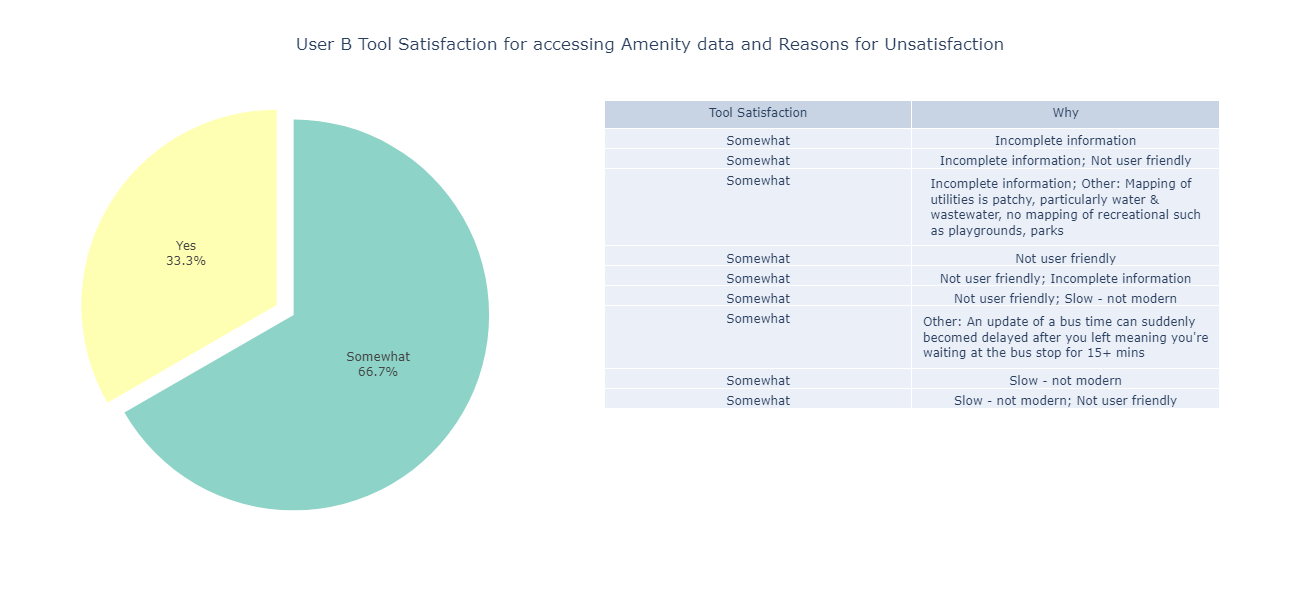
\includegraphics[width=0.8\textwidth]{images/mr-userb-tool-satisfaction.png}
    \caption{Market analysis - User B Tool satisfaction \& Usage frequency}
\end{figure}

\subsubsection{Thoughts on Magpie}
Lastly, this section covers questions regarding Magpie's potential to bridge the
gap in modern visualizing solutions.

%magpie usefulness user a
\begin{figure}[htbp]
    \centering{}
    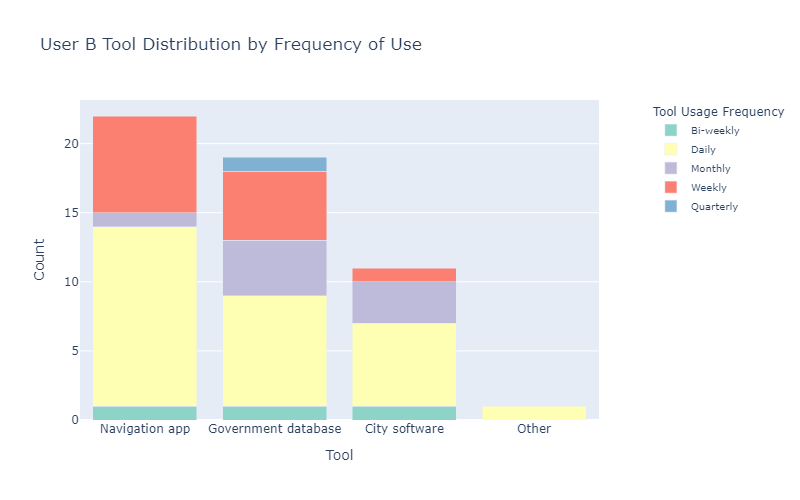
\includegraphics[width=0.8\textwidth]{images/mr-userb-tool-freq.png}
    \caption{Market analysis - User A Thoughts on Magpie}
\end{figure}

%magpie usefulness user b
\begin{figure}[htbp]
    \centering{}
    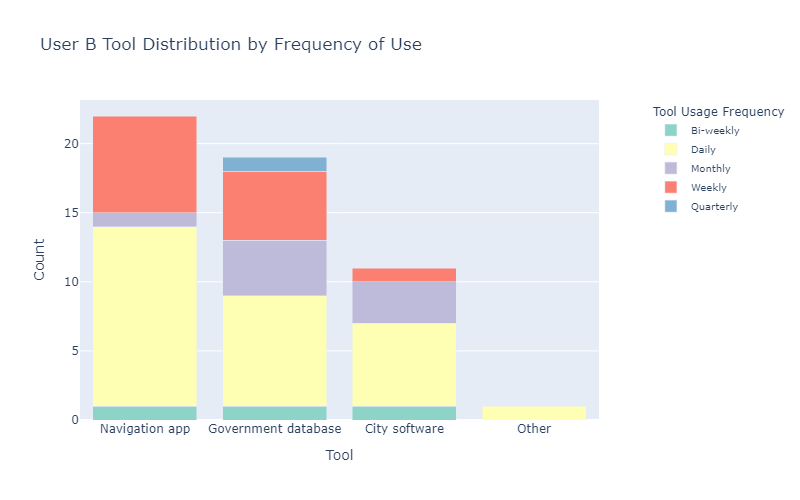
\includegraphics[width=0.8\textwidth]{images/mr-userb-tool-freq.png}
    \caption{Market analysis - User B Thoughts on Magpie}
\end{figure}

Both user groups found that Magpie would be useful to access amenity data, less
than 5\% citing it would be impractical because either they did not require
access to this information, or other tools such as Google Maps already satisfied
their needs.

Users from group B were also asked what additional features they would like to
see on Magpie. The highest rated ones were a \textbf{search functionality} and
\textbf{filters}.

%magpie usefulness user b
\begin{figure}[htbp]
    \centering{}
    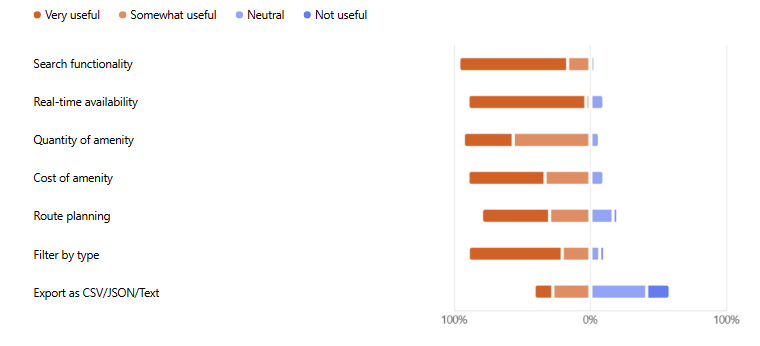
\includegraphics[width=0.8\textwidth]{images/mr-extra-features.png}
    \caption{Market analysis - User B Rating Additional Features}
\end{figure}

\textbf{Overall}, this exploratory work allows us to confirm our primary and
secondary target users as \emph{urban planners} and \emph{Non-Expert Users}
respectively.

Additionally, it gave us insight into a feature list to implement throughout
development, as well as competitors to research into.